\documentclass{article}
\usepackage[margin=0.65in]{geometry}
\usepackage{enumitem}
\usepackage{graphicx}
\usepackage{hyperref}
\usepackage{titlesec}
\usepackage{xcolor}
\hypersetup{hidelinks}
\setlist[itemize]{leftmargin=1.5em,topsep=2pt,itemsep=1pt,parsep=0pt,partopsep=0pt}
\titlespacing*{\section}{0pt}{1.2ex}{0.6ex}
\setlength{\parindent}{0pt}
\setlength{\parskip}{0.5em}
\setlength{\textfloatsep}{8pt}
\setlength{\intextsep}{6pt}
\setlength{\abovecaptionskip}{4pt}
\setlength{\belowcaptionskip}{0pt}
\makeatletter
\renewcommand{\maketitle}{%
    \begin{center}
        {\Large\bfseries \@title\par}\vspace{0.1em}
        {\normalsize \@author\par}\vspace{0.1em}
        {\small \@date\par}
    \end{center}\vspace{0.4em}
}
\makeatother
% HJNotes-Tags: AI Infra, Decoding Method, Sampling, Top-K
% HJNotes-Summary: Classical LLM decoding/sampling methods (greedy, beam, stochastic, top-k, top-p), how temperature reshapes logits, and the per-method sorting cost.
% AGENT WARNING: Polish task shouldn't delete or add new stuff unless there are serious mistake. typo should be fixed at once, permission is not needed.
\title{LLM Sampling Methods}
\author{HJ}
\begin{document}
\maketitle
% AGENT WARNING: only translate and polish the literal content, don't delete or add new stuff unless there are serious mistake.
\section{Introduction}
For LLM output there are lots of decoding methods, each deciding how to pick the next token from the model's output distribution.

\textbf{Terminology}: \underline{deterministic search} and \underline{stochastic sampling} are both \emph{decoding} methods. Since beam search is now rarely used, people often say ``sampling'' to mean the whole decoding category (even in vLLM/SGLang); be aware of the scope when reading.
\begin{figure}[!ht]
    \centering
    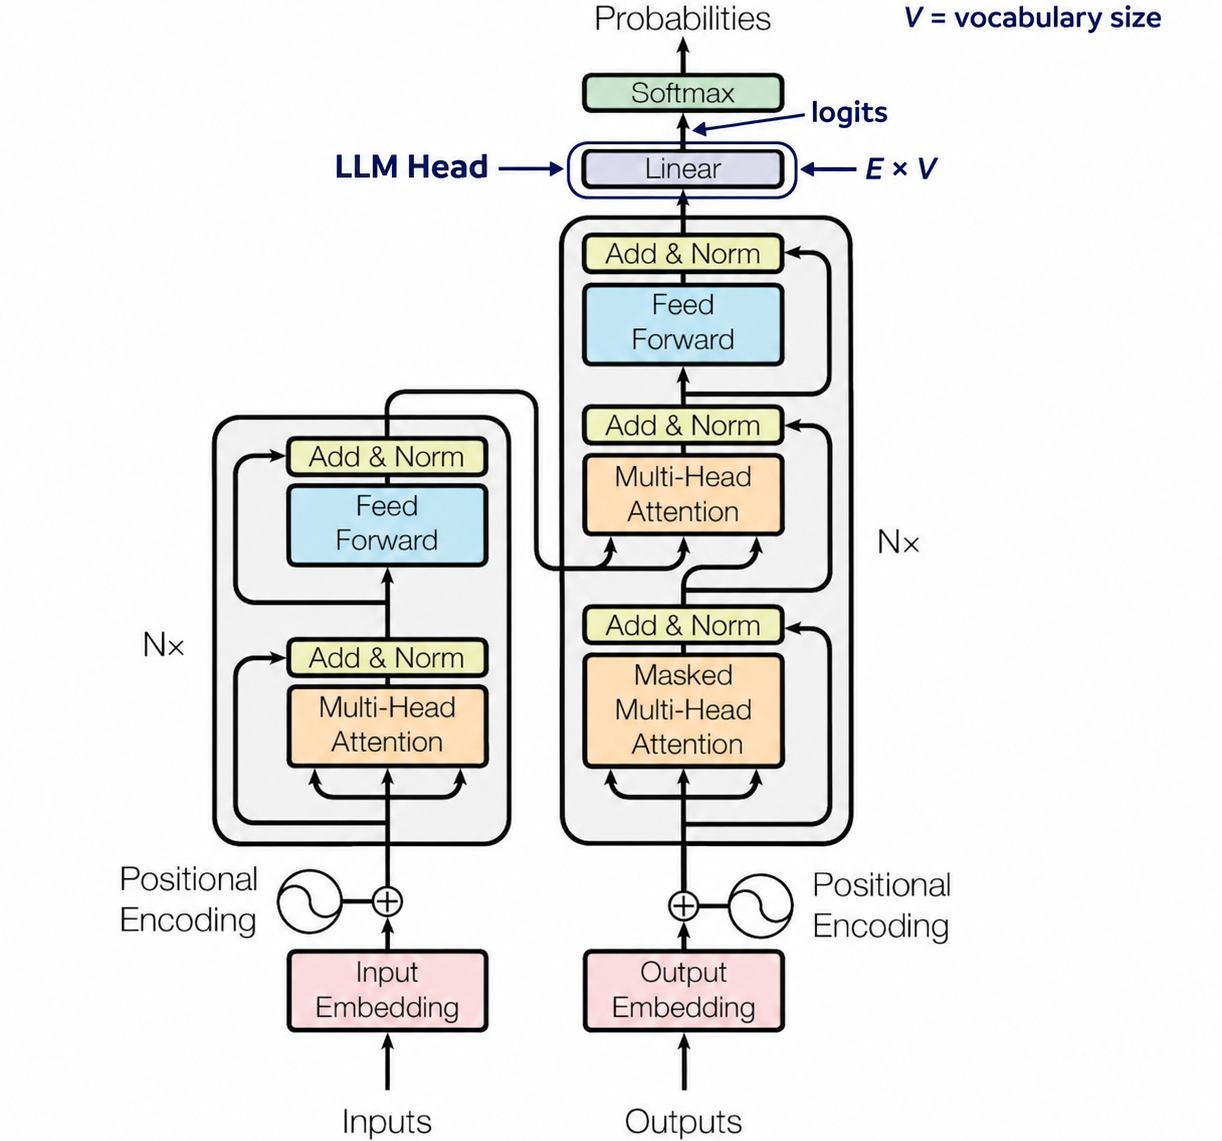
\includegraphics[width=0.59\linewidth,height=\textheight,keepaspectratio]{llm-head-annotated.png}
    \caption{LLM Head Structure}
\end{figure}

\section{Deterministic Search}
\begin{itemize}
    \item \textbf{Greedy Search}: always pick the token with the highest probability (\textcolor{blue}{$\arg\max$ only, softmax is not needed since the order unchange}), i.e.\ deterministic decoding. \emph{Drawback:} tend to \textcolor{red}{repeat} because losing too much info.
    \item \textbf{Beam Search}: keep the top-$N$ most probable partial sequences, like $N$ beams advancing in parallel through a $V$-branch tree ($V$ = vocabulary size). \emph{Drawback:} still easily repetive, root case not solved.
\end{itemize}

\section{Stochastic Sampling}
\begin{itemize}
    \item \textbf{Pure Sampling}: sample the next token from the full softmax distribution over the entire vocabulary. \emph{Drawback:} the \textcolor{red}{long tail} jointly carry non-trivial mass, so pure sampling often yields degenerate text.
    \item \textbf{Top-K Sampling}: keep only the $K$ highest-probability tokens, renormalize, then sample. \emph{Drawback:} \textcolor{red}{fixed rigid $K$}.
    \item \textbf{Top-P (Nucleus) Sampling}: keep the smallest set of tokens whose cumulative probability reaches $p$, renormalize, then sample; \textcolor{blue}{the cutoff adapts to the distribution.} \emph{Drawback:} still rigid truncation.
    \item \textbf{Min-P Sampling}: keep tokens with probability $\ge p\times \max(p_i)$, renormalize, then sample. Stabler under high temperature. \emph{Drawback:} don't know how to decide threshold, vLLM/SGLang didn't provide default value till now.
\end{itemize}

\textbf{Temperature} Factor $\tau$ rescales the logits $z_i$ before softmax, $p_i = \frac{\exp(z_i/\tau)}{\sum_{j}\exp(z_j/\tau)}$, Obviously:
\begin{itemize}
    \item $\tau < 1$ sharpens the distribution (shrinks the tail; \textcolor{blue}{$\tau \to 0$ approaches greedy,} which is a common implementation).
    \item $\tau = 1$ leaves it unchanged.
    \item $\tau > 1$ flattens it (spreads mass into the tail; $\tau \to \infty$ approaches uniform).
\end{itemize}
Unlike top-$k$/top-$p$, temperature never zeroes out a token --- it softly reweights but does not cut the tail.

\section{Summary}
Top-$p$ sampling needs probabilities \emph{fully sorted} (descending) to accumulate the cutoff; top-$k$ sampling and beam search only need \emph{partial sorted} (top-$K$ selection). Bitonic Sort is a powerful method for these sampling methods.

There are also other decoding type like \textbf{Speculative Decoding} for speed, and \textbf{Constrained Decoding} for structured output; but they are quite complex and different, need large infrastructure, deserving separate essay to discuss.

\begin{thebibliography}{1}
    \bibitem{hf-how-to-generate}
    P. von Platen, \emph{How to generate text: using different decoding methods for language generation with Transformers}, Hugging Face Blog, 2020, \href{https://huggingface.co/blog/how-to-generate}{huggingface.co/blog/how-to-generate}.
\end{thebibliography}

\end{document}

